% vim: set tw=0:
\documentclass{beamer}
\usepackage{graphicx}
\usepackage{hyperref}
\hypersetup{pdfborder={0 0 0 0}}

% Reasonable themes:
% Antibes Bergen Berkeley Berlin Frankfurt Goettingen Ilmenau Luebeck Malmoe
% Montpellier PaloAlto Rochester Singapore Szeged Warsaw bars boxes
% compatibility default lined plain shadow sidebar split tree
% And these ones include the author's name on every slide:
% Berkeley

% Declare themes.
\mode<presentation>
\usetheme{UWHEP}

% Personal macros.
\newcommand{\email}[1]{{\texttt #1}}
\newcommand{\newframe}[1]{\section{#1}
    \frametitle{\sc{#1}}}
\newcommand{\subframe}[1]{\subsection{#1}
    \frametitle{\sc{#1}}}
\newcommand{\supers}[1]{\ensuremath{^\textrm{#1}}}
\newcommand{\subs}[1]{\ensuremath{_\textrm{#1}}}
\newcommand{\ca}{\ensuremath{\sim}}
\renewcommand{\email}[1]{\href{mailto:#1}{\nolinkurl{#1}}}

% Author information.
\title{T2 Status}
\author[Maier, Mohapatra]{
    Will Maier \and Ajit Mohapatra\\
    {\tt wcmaier@hep.wisc.edu}\\
    {\tt ajit@hep.wisc.edu}}
\institute[Wisconsin]{University of Wisconsin - High Energy Physics}
\date{2010.05.11}
\logo{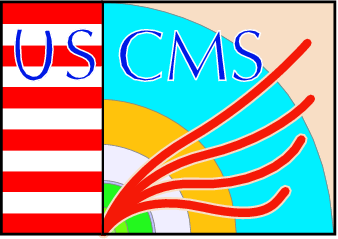
\includegraphics[height=0.6cm]{../../../Graphics/USCMS_logo.png}\hspace{.1cm}
\includegraphics[height=0.75cm]{../../../Graphics/UW_logo.png}}

\begin{document}

\begin{frame}
    \titlepage
\end{frame}

%\section{Overview}
%\begin{frame}
%    \tableofcontents
%\end{frame}

\section{Facilities}
\subsection{Software and Storage}
\begin{frame}
\frametitle{}

\begin{itemize}
	\item dCache: a series of unfortunate events
	\begin{itemize}
		\item Ran out of space, but couldn't account for all of it
		\item Local users quickly ramped up their analysis, wrote lots of PhEDEx data
		\item New workflows with lots and lots of small (tens of KB) files
		\item dCache pools became unstable (between 10 - 15\% offline each day)
		\item Pools become unstable when there are lots of queued requests (one thread per request?)
		\item Discovered bug in {\tt billingrep} that (seems to have) led to over replication, many simultaneous p2p transfers
		\item Testing to see if fix improves overall health
		\item Developed new system and dCache monitoring tools during debugging; plan to add DBS-vs-PNFS consistency check
	\end{itemize}
	\item Received test machine for next CPU purchase
\end{itemize}
\end{frame}

\subsection{Production and Monitoring}
\begin{frame}
\frametitle{}

\begin{itemize}
	\item JobRobot: dCache issues
	\item SAM: dCache issues
	\item RSV: dCache issues
	\item PhEDEx:
	\begin{itemize}
		\item Stable 3\_3\_0 on both Prod and Debug (SL4), haven't been able to 3\_3\_1 on SL5 yet
		\item Production transfers are OK, but LoadTest has suffered due to dCache issues
	\end{itemize}
	\item MC Production:
	\begin{itemize}
		\item Spring10 production (preproduction, fullsim, fastsim, etc) in full swing
		\item No issues so far
	\end{itemize}
\end{itemize}
\end{frame}
\end{document}
